\documentclass[10pt,twocolumn,letterpaper]{article}

% Những thứ riêng của tôi
\usepackage{booktabs}
% \usepackage{caption}
% \captionsetup[table]{skip=8pt}   % Chỉ ảnh hưởng tới bảng
\usepackage{stfloats}  % Thêm dòng này vào phần tiền đề
\usepackage{float}
\usepackage[T5]{fontenc}
\usepackage[vietnamese]{babel}

\usepackage{cvpr}
\usepackage{times}
\usepackage{epsfig}
\usepackage{graphicx}
\usepackage{amsmath}
\usepackage{amssymb}

% Bao gồm các gói khác ở đây, trước hyperref.

% Nếu bạn bình luận hyperref rồi bỏ bình luận lại, bạn nên xóa
% egpaper.aux trước khi chạy lại latex.  (Hoặc chỉ cần nhấn 'q' vào lần chạy latex đầu tiên,
% để nó hoàn thành, và bạn sẽ rõ ràng).
\usepackage[breaklinks=true,bookmarks=false]{hyperref}

\cvprfinalcopy % *** Bỏ chú thích dòng này cho bài nộp cuối cùng

\def\cvprPaperID{****} % *** Nhập CVPR Paper ID tại đây
\def\httilde{\mbox{\tt\raisebox{-.5ex}{\symbol{126}}}}

% Các trang được đánh số trong chế độ gửi bài, và không đánh số trong bản camera-ready
%\ifcvprfinal\pagestyle{empty}\fi
\setcounter{page}{1}
\begin{document}

%%%%%%%%% TIÊU ĐỀ
\title{Sách giáo trình dữ liệu ECDO Phần 1/2: Hiểu biết hiện tại về Lý thuyết Dao động Tách Lõi-Manti Exo Nhiệt (ECDO) “Lật Trái Đất”}

\author{Junho\\
Xuất bản tháng 2 năm 2025\\
Website (Tải tài liệu ở đây): \href{https://sovrynn.github.io}{sovrynn.github.io}\\
ECDO Research Repo: \href{https://github.com/sovrynn/ecdo}{github.com/sovrynn/ecdo}\\
{\tt\small junhobtc@proton.me}
% Đối với một bài báo mà tất cả các tác giả đều ở cùng một tổ chức,
% hãy bỏ qua các dòng sau cho đến dấu ``}'' kết thúc.
% Các tác giả và địa chỉ bổ sung có thể được thêm vào với ``\and'',
% giống như tác giả thứ hai.
% Để tiết kiệm không gian, chỉ sử dụng địa chỉ email hoặc trang chủ, không sử dụng cả hai
% \and
% xxx
% Institution2\\
% Dòng đầu tiên của địa chỉ institution2\\
% {\tt\small secondauthor@i2.org}
}

\maketitle
%\thispagestyle{empty}

%%%%%%%%% TÓM TẮT
\begin{abstract}
Vào tháng 5 năm 2024, một tác giả ẩn danh trên mạng có tên là “The Ethical Skeptic” \cite{0} đã chia sẻ một lý thuyết đột phá có tên là Dao động Tách rời Vỏ-Lõi Ngoại Nhiệt ECDO (Exothermic Core-Mantle Decoupling Dzhanibekov Oscillation) \cite{1}. Lý thuyết này cho rằng Trái Đất trước đây đã từng trải qua những chuyển động đột ngột, thảm khốc của trục quay, gây ra những trận lụt lớn trên toàn thế giới khi đại dương tràn lên các lục địa do quán tính quay. Ngoài ra, lý thuyết này trình bày một quá trình địa vật lý giải thích cùng các dữ liệu cho thấy một lần lật trục như vậy có thể sắp xảy ra. Mặc dù các dự đoán về trận lụt tận thế và ngày tận thế không phải là mới, lý thuyết ECDO lại đặc biệt thuyết phục nhờ cách tiếp cận khoa học, hiện đại, đa ngành và dựa trên dữ liệu.

This paper is the first part of a two-part condensed summary of six months of independent research \cite{2,20} into the ECDO theory. It highlights three key points:

\begin{flushleft}
\begin{enumerate}
    \item Một sự kiện 'Lật Trái Đất' tương tự ECDO đã xảy ra nhiều lần trong lịch sử gần đây của loài người, được chứng minh bởi các thần thoại về trận đại hồng thuỷ và các dấu hiệu địa chất về lụt lội diện rộng trên các lục địa.
    \item Hướng và độ lớn xấp xỉ của các lần lật Trái Đất trong quá khứ có thể xác định được.
    \item Các dữ liệu địa từ và địa vật lý gần đây cho thấy rằng một sự kiện lật Trái Đất nữa có thể sắp xảy ra, và biến đổi khí hậu có thể là do những thay đổi sâu bên trong Trái Đất chứ không phải do con người gây ra.
\end{enumerate}
\end{flushleft}

Ngoài ra, tôi trình bày các cơ sở vật lý gây ra hiện tượng “lật Trái Đất” được đề xuất bởi lý thuyết ECDO.

Trong bài báo này, tôi giữ thái độ khách quan bằng cách tập trung vào dữ liệu thực nghiệm, tránh các phần ấn tượng nhưng còn mang tính suy đoán của lý thuyết, và nhấn mạnh rằng đây là chủ đề mà nhân loại cần cấp thiết nghiên cứu thêm.
\end{abstract}

%%%%%%%%% BODY TEXT
\section{Giới thiệu}

Các câu chuyện về trận đại hồng thuỷ không phải là điều mới mẻ - thực tế, chúng xuất hiện trong mọi nền văn hoá lớn trên toàn cầu, trải rộng khắp các cái nôi của nền văn minh. Việc minh hoạ (Hình \ref{fig:1}) một tổng hợp 267 câu chuyện về lũ lụt \cite{3} cho thấy hầu như tất cả các khu vực có người sinh sống trên Trái Đất đều có truyền thuyết về lũ lụt.
```
% \begin{figure}[h]
% \begin{figure}[b]
\begin{figure}[h]
\begin{center}
% \fbox{\rule{0pt}{2in} \rule{0.9\linewidth}{0pt}}
   \includegraphics[width=1\linewidth]{b.png}
\end{center}
   \caption{Vị trí các câu chuyện về lũ lụt trên khắp thế giới \cite{3}.}
\label{fig:1}
\label{fig:onecol}
\end{figure}

Một cái nhìn kỹ hơn về các câu chuyện lũ lụt này cho thấy đây không phải là những trận lụt thông thường, mà là các thảm họa mang tính hủy diệt kèm theo lũ lụt đã quét sạch các lục địa.

\subsection{Các câu chuyện về thảm họa của người Mỹ bản địa}

Các câu chuyện của người Mỹ bản địa chứa đựng một số ghi chép sống động nhất về những thảm họa lớn của Trái Đất. Người Hopi, một bộ tộc người Mỹ bản địa sống ở đông bắc Arizona, nói rằng, \textit{"..Sótuknang đã kêu gọi người Kiến mở cánh cửa dẫn vào thế giới dưới lòng đất cho những người được chọn. Khi họ an toàn dưới lòng đất, Sótuknang ra lệnh cho cặp song sinh, Pöqánghoya và Palöngawhoya, rời vị trí ở hai đầu bắc và nam của trục Trái Đất, nơi họ được giao nhiệm vụ giữ cho Trái Đất quay đúng cách. \textbf{Cặp song sinh vừa rời khỏi vị trí thì thế giới, không còn ai kiểm soát, lảo đảo mất cân bằng, quay cuồng điên dại, rồi lộn nhào hai lần.} Những ngọn núi lao xuống biển với tiếng động lớn, biển và hồ nước tràn lên đất liền; và khi thế giới quay qua không gian lạnh lẽo, không sự sống, nó đóng băng thành băng rắn"} \cite{4}.

Nhiều câu chuyện trong số này miêu tả chính xác quy mô khổng lồ của trận lụt, kể lại rằng các đại dương đã dâng lên nhấn chìm tất cả trừ những đỉnh núi cao nhất. Người Skokomish, sống ở bang Washington, kể rằng, \textit{"Đại Linh Hồn, tức giận vì sự xấu xa của con người và thú vật, quyết định loại bỏ Trái Đất khỏi tất cả trừ những con vật tốt, một người đàn ông tốt và gia đình ông. Theo chỉ dẫn của Đại Linh Hồn, người đàn ông bắn một mũi tên lên mây, rồi tiếp tục bắn mũi tên vào mũi tên đó, tiếp tục như vậy, tạo thành một sợi dây bằng tên từ mây xuống mặt đất. Những con vật và người tốt đã trèo lên. Các loài vật xấu và rắn cũng bắt đầu trèo lên, nhưng người đàn ông đã bẻ gãy sợi dây tên đó. \textbf{Sau đó, Đại Linh Hồn gây ra nhiều ngày mưa, lũ lụt dâng lên đến tận ranh giới tuyết của Takhoma (núi Ranier).} Sau khi những người xấu và vật xấu bị chết đuối hết, Đại Linh Hồn dừng mưa, nước dần rút xuống, và người tốt và vật tốt đã trèo xuống"} \cite{3}. Để tham khảo, núi Rainier là một núi lửa đang hoạt động ở Washington với độ cao đỉnh 4392,5 m so với mực nước biển.
```
Câu chuyện về trận lụt của người Makah ở bang Washington đặc biệt đề cập đến một trận lụt nhiều giai đoạn với nước "rất ấm", cho thấy đây không phải là một trận lụt bình thường: \textit{"Biển dâng cao đủ để cắt đứt mũi đất. Sau đó biển rút đi, đạt mức thấp nhất sau bốn ngày, để lại Vịnh Neah khô ráo. Rồi nó lại dâng lên, bao phủ tất cả trừ các đỉnh núi. \textbf{Nước dâng lên rất ấm.} Những người có xuồng chất đồ đạc của họ và bị cuốn trôi xa về phía bắc. Nhiều người đã chết khi xuồng của họ bị mắc vào cây. Biển trở lại bình thường sau bốn ngày nữa, và mọi người nhận ra mình đang ở xa về phía bắc, nơi con cháu của họ vẫn còn sống đến nay"} \cite{3}.

\subsection{Những câu chuyện đại nạn của Trung Hoa}

Ở phía bên kia Thái Bình Dương, nền văn minh Trung Hoa hiện đại được cho là bắt đầu từ một trận đại hồng thuỷ. Triều đại Hạ, được ước tính tồn tại vào khoảng năm 2000 TCN, được lập nên bởi Đại Vũ, người đã dập tắt trận Đại hồng thủy của Cống và Vu \cite{6}. Thời ông, \textit{"... phép lạ được cho là đã xảy ra khi mặt trời suốt mười ngày không lặn, rừng núi bốc cháy, và vô vàn loài côn trùng ghê tởm xuất hiện... Một con sóng khổng lồ “chạm tới trời” đã đổ ập xuống đất Trung Hoa. \textbf{"Nước dâng cao tới tận các ngọn núi, chân núi thì không thể nhìn thấy"}... "Nước lũ tràn lan thật tàn phá," hoàng đế nói. "Chúng mênh mông ôm trọn những ngọn đồi và vượt lên đỉnh cao, dọa dẫm trời bằng nước lũ." Hoàng đế ra lệnh phải tìm mọi cách mở đường cho nước thoát ra khỏi các thung lũng giữa núi. Trong nhiều năm dân chúng vất vả làm việc, cố gắng khai thông đồng bằng và thung lũng khỏi nước bằng cách đào kênh và tiêu nước trên đồng ruộng. Trong một thời gian dài mọi nỗ lực đều vô ích. Vị đại thần chịu trách nhiệm cho công việc to lớn và cấp bách này, Khwan, đã bị xử tử vì thất bại... và chỉ có con trai ông là Vũ mới thành công trong việc tiêu nước lũ. Thành tựu ấy được đánh giá rất cao nên Vũ đã trở thành hoàng đế Trung Hoa sau vua Thuấn, người kế vị đầu tiên của Nghiêu"} \cite{5}.

Dường như không chỉ có Trung Hoa bị lụt, mà thậm chí còn phải đo lại các hướng chính và chuyển động của mặt trời và mặt trăng, cho thấy có thể Trái đất đã thay đổi chuyển động quay trong trận lụt: \textit{\textbf{"Vị hoàng đế này đã cử các học giả đến nhiều nơi trên đất Trung Hoa, thậm chí cả đến Đông Dương, để xác định vị trí của bắc, tây, đông và nam bằng cách quan sát hướng mặt trời mọc và lặn và chuyển động của các vì sao.} Ông ta cũng giao nhiệm vụ cho các nhà thiên văn xác định độ dài các mùa và lập lịch mới... "Do đó Nghiêu [Yahou] sai Hề và Hoà, một cách kính cẩn tuân theo mệnh trời, tính toán và mô tả chuyển động cũng như hình dạng của mặt trời, mặt trăng, các vì sao và các chòm sao hoàng đạo; và tôn trọng phân chia thời tiết cho dân chúng""} \cite{5}.

Các ghi chép về đại nạn trong lịch sử Trung Hoa thực ra còn có từ xa trước thời Hạ, thậm chí từ thời kỳ Tam Hoàng Ngũ Đế \cite{7}. Nữ Oa, một trong Tam Hoàng và là nhân vật Sáng Tạo trung tâm trong lịch sử Trung Hoa, đã ngăn lụt trong một đại họa mà Trái đất bị đổi hướng quay: \textit{"Có cuộc tranh cãi giữa hai vị thần quyền năng hơn, và họ quyết định giải quyết bằng trận chiến. Khi thần nước Cộng Công thấy mình thất bại, ông đã dùng đầu húc vào núi Bất Chu, cây cột chống trời. \textbf{Cây cột bị sập khiến trời nghiêng về tây bắc, đất dạt về đông nam.} Hậu quả là xảy ra đại họa: lửa cháy dữ dội, nước lụt tràn lan, và có những con thú dữ ăn thịt người xuất hiện. Nữ Oa cắt chân một con rùa khổng lồ dùng làm cột thay cho cột bị sập, làm dịu tình hình và vá trời bằng bảy màu đá khác nhau, nhưng bà không thể hoàn toàn sửa được trời nghiêng"} \cite{8}.

\subsection{Những câu chuyện đại nạn của châu Âu, Maya, Trung Đông và Đông Nam Á}

Vì có quá nhiều chuyện đại họa để kể chi tiết trong bài viết này, tôi sẽ chỉ đề cập ngắn gọn về một số nền văn hóa tiêu biểu khác có các câu chuyện tương tự. Văn học Hy Lạp có ba chuyện lụt, đó là của Deucalion, Ogyges, và Dardanus \cite{9,10}. Trong chuyện thứ nhất, \textit{"Sau chín ngày lụt, thế giới bị hủy diệt, và chiếc thuyền dừng lại trên đỉnh núi Parnassus"}, đỉnh núi này cao 2.457 mét \cite{11}. Văn học Maya tin rằng đã có bốn Mặt trời khác nhau trước Mặt trời hiện tại, và kỷ nguyên của Mặt trời thứ tư, Calchiuhtlicue, kết thúc bằng một trận đại hồng thủy phá hủy thế giới khoảng năm 3100 TCN cùng với sự ra đời của Mặt trời thứ năm hiện tại \cite{12}. Ở Trung Đông, niên đại Kinh Thánh ghi lại trận Đại Hồng thủy nổi tiếng của Nô-ê, và Sử thi Gilgamesh, một trường ca Babylon, cũng kể lại câu chuyện tương tự \cite{13}. Các nền văn hóa Đông Nam Á cũng rất giàu truyền thuyết về lụt - ví dụ, người Ot Danum ở Indonesia kể rằng, \textit{"Một trận đại hồng thủy từng nhấn chìm rất nhiều người. Một số ít sống sót bằng cách chạy trốn trên thuyền tới đỉnh núi duy nhất còn nhô lên khỏi mặt nước. Họ trú ngụ ở đó ba tháng cho đến khi nước rút"} \cite{3}. Đảo Borneo, nơi họ sinh sống, có đỉnh cao nhất là 4.095 mét.

\begin{figure*}[b]
\begin{center}
% \fbox{\rule{0pt}{2in} \rule{.9\linewidth}{0pt}}
\includegraphics[width=1\textwidth]{marine.jpg}
\end{center}
   \caption{Bản đồ toàn cầu về hóa thạch biển (đại dương), nước mặn và các bãi muối/mỏ muối \cite{15,16,86,87}.}
   \label{fig:2}
\end{figure*}

\subsection{Phân Tích Thống Kê Các Câu Chuyện Đại Họa}

Rõ ràng, những câu chuyện này miêu tả các trận đại hồng thủy thường đi kèm với các loại lực địa chất tai họa khác. Phân tích 117 câu chuyện đại họa (Bảng \ref{tab: 1}) cho thấy rằng các trận bão lửa, thay đổi địa hình, và thay đổi chuyển động quay của Trái Đất thường được ghi lại là xảy ra cùng với các trận đại hồng thủy lớn \cite{14}:

\begin{table}[ht]
\begin{center}
\renewcommand{\arraystretch}{1.2}  % Optional, to increase row spacing
\begin{tabular}{|l|c|c|}
\hline
\textbf{Loại Đại Họa} & \textbf{Số Lượng} & \textbf{Tỉ Lệ Xuất Hiện \%} \\
\hline\hline
Đại hồng thủy/lũ lụt            & 84 & 71.79 \\
Hỏa hoạn/bão lửa                & 39 & 33.33 \\
Thay đổi địa hình               & 29 & 24.79 \\
Nhiễu loạn thiên thể            & 15 & 12.82 \\
Bầu trời sụp xuống              & 15 & 12.82 \\

Prolonged darkness      & 14 & 11.97 \\
Đất và hồ bị mất        & 12 & 10.26 \\
Gió xoáy                 & 10 & 8.55  \\
Thay đổi trục/quay      & 9 & 7.69  \\
Sông/hồ/đại dương sôi    & 8 & 6.84 \\
\hline
\end{tabular}
\end{center}
\caption{Tần suất xuất hiện các tác động thảm khốc trong truyện kể}
\label{tab: 1}
\end{table}

Tính đặc thù của các truyện kể về lũ lụt xuất hiện ở nhiều nền văn hóa độc lập trên khắp thế giới, cùng với các câu chuyện tương đồng về những hiện tượng thảm họa khác, cho thấy rằng những câu chuyện này có thể là những ghi chép trực tiếp về các thảm họa thực sự đã xảy ra.

\section{Bằng chứng vật lý về trận lụt đại dương}

Ủng hộ các truyện kể về lũ lụt là nhiều hình thái bằng chứng vật lý về sự ngập nước đại dương trên diện rộng nằm trên bề mặt các lục địa của Trái Đất. Dạng bằng chứng trực tiếp nhất bao gồm muối (nước mặn, ruộng muối, và mỏ muối) và hóa thạch sinh vật biển, những thứ bao phủ những khu vực rộng lớn trên lục địa của Trái Đất. Hình \ref{fig:2} thể hiện sơ đồ nước mặn (màu xanh), ruộng/mỏ muối (màu nâu), và hóa thạch sinh vật biển \cite{15,16,86,87}, minh họa phạm vi của các dấu hiệu ngập nước đại dương này.

Một số khu vực thú vị nhất chứa nước mặn là vùng cao nguyên Himalaya ở Tây Tạng và dãy Andes ở Nam Mỹ, cả hai khu vực đều có độ cao trung bình 4000 mét, khu vực Tây Tạng được thể hiện trong hình \ref{fig:3}. Các truyền thuyết về lũ lụt ở Tây Tạng kể rằng, \textit{"\textbf{Tây Tạng đã gần như hoàn toàn chìm trong biển nước}, cho đến khi thần Gya thương cảm những người sống sót, rút nước qua Bengal, và gửi các vị thầy đến dạy dỗ dân chúng, những người trước đó sống chẳng khác gì loài khỉ"} \cite{3}. Thần thoại Peru mô tả việc hình thành núi diễn ra cùng lúc với trận lụt bao phủ đỉnh núi: \textit{"Người chăn cừu và sáu đứa con tập hợp mọi thức ăn và cừu có thể và đưa chúng lên đỉnh núi rất cao tên là Ancasmarca. \textbf{Khi nước lũ dâng lên, ngọn núi cũng trồi cao hơn, nên đỉnh của núi không bao giờ bị ngập, và núi này sau đó chìm xuống cùng với nước.} Sáu đứa trẻ đó đã làm dân số lại cho vùng này sau trận lụt."} \cite{3}.
\begin{figure}[t]
\begin{center}
% \fbox{\rule{0pt}{2in} \rule{0.9\linewidth}{0pt}}
   \includegraphics[width=1\linewidth]{tibet.jpg}
\end{center}
   \caption{Bản đồ địa hình của dãy Himalaya thể hiện nước muối (màu xanh ngọc), muối khô (màu trắng), và hóa thạch sinh vật biển (màu đỏ) \cite{15,16,86,87}.}
\label{fig:3}
\label{fig:onecol}
\end{figure}

Trong khi trường phái đồng nhất trong tư tưởng địa chất cho rằng các hiện tượng bất thường như muối và hóa thạch sinh vật biển là kết quả của các quá trình kéo dài hàng triệu năm, các câu chuyện về trận đại hồng thủy của nhân loại nên khiến chúng ta đặt câu hỏi về hướng suy nghĩ đó. Nếu thực sự đại dương đã ngập tràn các lục địa, thì nước muối và hóa thạch sinh vật biển, dễ dàng được phát hiện trên những vùng đất cao rộng lớn, chính là điều mà chúng ta mong đợi sẽ tìm thấy.

\begin{figure*}[t]
\begin{center}
\includegraphics[width=0.85\textwidth]{khafre.jpg}
\end{center}
   \caption{Sơ đồ cho thấy sự xói mòn karst có tính phân hóa, có hoa văn, gây ra bởi sự dâng lên tạm thời và kéo dài của mực nước biển \cite{27}.}
\label{fig:4}
\end{figure*}
\subsection{Các Dị Thường Vật Lý Bổ Sung}

Có rất nhiều dạng dị thường khác mà khoa học đồng nhất không thể giải thích. Những con voi ma mút được cấp đông siêu nhanh, còn nguyên vẹn, bị chôn vùi trong bùn với thịt vẫn còn ăn được sau hàng nghìn năm \cite{17,18,19}, các lớp trầm tích khổng lồ được xếp chồng lên nhau theo chiều ngang ở Bắc Mỹ trải dài trên diện tích 2.4 triệu km$^2$ \cite{21}, các cảnh quan gợn sóng dòng siêu lớn \cite{22}, và các tảng đá lạc xuất phát từ hàng trăm kilômét xa xôi nằm trên đỉnh núi \cite{23,26} chỉ là một số hiện tượng mà địa chất học đồng nhất hiện đại chỉ đưa ra những giải thích cẩu thả bằng cụm từ “quy trình kéo dài lâu dài”. Những dị thường như vậy được giải thích hợp lý nhất thông qua các lực địa vật lý mang tính thảm họa, và sẽ được bàn sâu hơn ở phần hai của bài báo này.

Ngoài ra, các lần dịch chuyển và đảo ngược cực từ địa từ được công nhận rộng rãi là các hiện tượng lặp lại của Trái Đất, dựa trên dữ liệu cổ địa từ \cite{35,40,41}. Tuy nhiên, khoa học hiện đại lại chưa thể giải thích chính xác tại sao và bằng cách nào các sự đảo cực này xảy ra.

\section{ECDO và các Kim Tự Tháp Giza}

Kim tự tháp Khafre và Khufu tại Giza là một trong những điểm tập trung chính trong luận thuyết ECDO của Ethical Skeptic \cite{27}, vì chúng không chỉ cung cấp bằng chứng về một trận lũ tạm thời kéo dài từ đại dương mà còn gợi ý hướng dịch chuyển tiềm năng của các lần lật ECDO của Trái Đất, cho thấy tổ tiên chúng ta đã có khả năng đo đếm các thảm họa của Trái Đất và có kỹ năng xây dựng để tích hợp kiến thức này vào các công trình đá khổng lồ được kỹ thuật hóa cao. Hai kim tự tháp này, theo giả thuyết được xây dựng khoảng năm 2500 TCN để làm lăng mộ cho các pharaon Khufu và Khafre, đều nằm ở phía bắc Ai Cập tại khoảng (30 N, 31 E). Chúng có đáy dài hơn 200 mét, và cao khoảng 140 mét. Kim tự tháp Khufu được xây dựng từ khoảng 2,3 triệu khối đá vôi, mỗi khối nặng trung bình trên hai tấn \cite{24, 25}.

Có rất nhiều sự không chắc chắn liên quan đến nguồn gốc của các kim tự tháp này, vấn đề mà Ethical Skeptic cũng đề cập trong luận thuyết của mình. Ông chỉ ra nhiều điểm bất nhất trong câu chuyện truyền thống về các kim tự tháp, cho thấy, ít nhất, có sự nhầm lẫn lớn về tuổi thọ và lịch sử của các công trình này:

\begin{flushleft}
\begin{itemize}
    \item Kết quả định tuổi bằng carbon đối với các loại vữa cổ đại và công cụ đào trộm lăng mộ gần đó cho thấy các kim tự tháp có thể được xây dựng sớm hơn rất nhiều so với nhận định truyền thống.
    \item Các “dấu mỏ đá” được cho là tìm thấy trong các phòng bên trong kim tự tháp Khufu có nhiều điểm nghi vấn về vị trí, chất liệu, mức độ bảo quản, cách sử dụng chữ tượng hình Ai Cập, cũng như thời điểm và bản chất phát hiện, cho thấy chúng có thể là giả mạo. Ngoài ra, chúng cũng khác biệt so với các vết đánh dấu bằng màu đỏ son thật sự cổ xưa khác được tìm thấy ở phần khác của kim tự tháp.
    \item Hiện tượng ăn mòn karst khác biệt trên tượng Nhân sư gần đó không phù hợp với câu chuyện truyền thống về quá trình xây dựng của nó.
\end{itemize}
\end{flushleft}
\begin{figure*}[b]
\begin{center}
\includegraphics[width=0.85\textwidth]{shafts.jpg}
\end{center}
   \caption{Các giếng và buồng bên trong của Kim tự tháp Khufu, mà Ethical Skeptic đề xuất là một đài quan trắc địa vật lý ba phần cho các sự kiện ECDO \cite{28}.}
\label{fig:5}
\end{figure*}

Một trong những lĩnh vực điều tra trọng yếu trong luận đề của Ethical Skeptic là hiện tượng xói mòn khác biệt, có quy luật trên bề mặt ngoài của Kim tự tháp Khafre, được minh họa tại Hình \ref{fig:4}. Đỉnh của kim tự tháp vẫn giữ được phần vỏ ngoài bằng đá vôi Tura mềm nguyên bản, từng bao phủ toàn bộ kim tự tháp. Đỉnh ốp đá vôi này bị phong hóa nhẹ, nhưng nằm ngay phía trên một lớp đá bị xói mòn karst mạnh và hẹp, làm lộ ra lớp đá vôi Mokkatam cứng hơn (Mohs 7) dùng cho các khối kết cấu bên trong kim tự tháp. Dưới đó, thân của kim tự tháp giữ lại một lớp đá vôi Tura (Mohs 4) bị xói mòn karst mạnh. Điểm then chốt ở đây là đá vôi Tura mềm dùng cho vỏ ngoài kim tự tháp, có thành phần là CaCO$_3$, có thể bị hòa tan trong nước trong điều kiện thích hợp. Ethical Skeptic trích dẫn rằng lớp xói mòn karst mạnh có chọn lọc dừng lại ở đá vôi Mokkatam cứng, các hoa văn xói mòn dạng sóng ở các góc của đỉnh kim tự tháp, và sự khác biệt giữa quá trình phong hóa nhẹ ở đỉnh cao và xói mòn karst mạnh ở phần thân thấp của kim tự tháp là bằng chứng rõ ràng cho một đợt dâng mực nước biển kéo dài và sau đó rút đi nhanh chóng \cite{27}.

\begin{figure*}[b]
\begin{center}
% \fbox{\rule{0pt}{2in} \rule{.9\linewidth}{0pt}}
\includegraphics[width=1\textwidth]{drawing.jpg}
\end{center}
   \caption{Minh họa xoay ECDO được đề xuất với góc 104 độ lên phía bắc dọc theo kinh tuyến 31 độ Đông, với các dấu thập thể hiện các điểm trụ phía đông và phía tây, và một dấu đỏ thể hiện vị trí Kim tự tháp Khufu.}
\label{fig:6}
\end{figure*}

Ethical Skeptic cũng tập trung mạnh vào thiết kế nội thất và tình trạng bên trong của kim tự tháp Khufu (Hình \ref{fig:5}) trong nghiên cứu của mình \cite{28}. Kim tự tháp Khufu có nhiều buồng (buồng Vua, buồng Hoàng hậu và buồng ngầm), các hành lang và giếng khác nhau, cũng như hai cặp gọi là “giếng thông gió”, với mỗi cặp xuất phát từ buồng Vua và buồng Hoàng hậu \cite{29,30}. Trong bài viết này, chúng tôi chỉ trình bày các phần quan trọng nhất trong nghiên cứu của Ethical Skeptic – đó là hướng và thiết kế của hai cặp “giếng thông gió”, vì những giếng này mã hóa thông tin quan trọng về hướng đảo cực ECDO của Trái Đất.
Điều then chốt ở đây là hiểu rằng các ống thông khí được xây dựng nhằm chỉ rất chính xác về một số hướng nhất định. Trước tiên, cả hai cặp ống hiện tại đều hướng thẳng về phía bắc và nam. Ngoài ra, chúng đều được xây dựng với một góc bên trong là 104 độ.

Tuy nhiên, manh mối rõ ràng nhất là một bản đồ sao thiên văn được khắc trên bề mặt bên trong của một trong các ống thông khí của Nữ hoàng. Bản đồ sao này tập trung vào hướng bắc thiên thể từ khoảng năm 9600 đến 9200 TCN, dựa trên sự tiến động của các điểm phân \cite{28}. Điều này gợi ý rằng có một sự định hướng có chủ ý của các ống thông khí, và vào thời điểm xây dựng, một cặp ống của các phòng vua và nữ hoàng đã chỉ về cực bắc thiên thể. Điều này đặt ra câu hỏi - đầu còn lại của các ống thông khí chỉ về đâu, và tại sao cả hai đều được xây dựng với một góc 104 độ? Ethical Skeptic đề xuất rằng những ống này được xây dựng nhằm trùng với cực bắc thiên thể sau một lần lật ECDO 104 độ.

\section{Bằng chứng cho Sự Quay 104 Độ Dọc Kinh Tuyến 31}

Ethical Skeptic do đó đưa ra giả thuyết rằng Trái Đất trải qua các lần lật 104 độ lặp đi lặp lại dọc theo kinh tuyến 31, theo đó Kim tự tháp Khufu và các ống thông khí kép của nó nằm. Hình \ref{fig:6} minh họa cho sự quay dự đoán, cùng với hai “trục" đông (Indonesia, 121 độ Đ) và tây (Nam Mỹ, 59 độ T), hai vị trí sẽ không thay đổi vị trí sau khi lật dọc theo kinh tuyến 31. Sau khi Trái Đất quay về trạng thái mới này, nó được dự đoán sẽ duy trì tình trạng này trong thời gian ngắn (vài thập kỷ đến thế kỷ) trước khi trở lại trạng thái "bình thường” hiện nay \cite{150}.

Một câu chuyện về thảm họa đặc biệt liên quan là do Herodotus, nhà sử học nổi tiếng nhất ở Hy Lạp cổ đại, người sống vào thế kỷ thứ năm TCN \cite{31}. Trong cuốn sách “Miêu tả về Ai Cập”, Herodotus kể lại rằng các tu sĩ Ai Cập đã kể cho ông: \textit{"...từ vị vua đầu tiên cho đến vị tu sĩ của Hephaistos trị vì cuối cùng, đã có ba trăm bốn mươi mốt thế hệ người... nhưng ba trăm thế hệ người bằng mười nghìn năm, bởi một trăm năm là ba thế hệ người... Như vậy, trong khoảng thời gian mười một nghìn ba trăm bốn mươi năm họ nói rằng không có vị thần nào xuất hiện dưới hình dạng con người; và cả trước đó hay sau này trong số các vị vua còn lại xuất hiện ở Ai Cập, họ cũng không báo cáo rằng có điều gì như vậy đã xảy ra. \textbf{Trong thời gian này, họ nói rằng mặt trời đã bốn lần di chuyển khỏi vị trí mọc quen thuộc, và tại nơi mà hiện tại nó lặn, nó đã hai lần mọc lên ở đó, và tại nơi mà hiện tại nó mọc, nó đã hai lần lặn ở đó;} và trong thời gian đó, không có gì ở Ai Cập bị thay đổi khỏi trạng thái thông thường, cả những gì đến từ đất hay những gì đến với họ từ sông, cũng như những gì liên quan đến bệnh tật hay cái chết"} \cite{32}. Vị tu sĩ của Hephaistos có thể được xác định vào đầu thế kỷ 7 TCN, vì ông là người cùng thời với Sennacherib, vị vua của Đế chế Tân Assyria, như chính Herodotus đã nói \cite{32,33,34}.

Câu chuyện này quan trọng vì nó cho chúng ta biết rằng khi mặt trời chuyển động ở Ai Cập, nó \textit{cụ thể đã đổi chỗ mọc và lặn}. Điều này chỉ có thể xảy ra nếu Ai Cập bị lật 180 độ và vẫn nằm trên vĩ độ tương tự. Khi tính đến thiết kế của các kim tự tháp và các dữ liệu trong phần tiếp theo, chúng ta có thể suy luận rằng Ai Cập nằm trên kinh tuyến mà Trái Đất quay về vị trí mới (kinh tuyến 31 Đông).

Ai Cập là \textit{nơi duy nhất} trên Trái Đất có câu chuyện kể rằng mặt trời đã cụ thể đổi chỗ mọc và lặn. Thực tế, câu chuyện duy nhất khác trên thế giới đề cập đến hướng quay cụ thể của Trái Đất là câu chuyện Nữ Oa của Trung Quốc, kể rằng, \textit{"Cột trụ sụp đổ khiến bầu trời nghiêng về tây bắc và mặt đất lệch về đông nam"} \cite{8}. Hướng quay này cũng trùng khớp với hướng quay được đề xuất.

\subsection{Bằng chứng vật lý cho sự quay 104 độ dọc kinh tuyến 31}

Bằng chứng vật lý ủng hộ hướng quay này bao gồm dữ liệu cổ từ về địa từ, kiến tạo, sa mạc, đa dạng sinh học, dòng chảy cổ, và các tảng đá trôi dạt do băng hà.

Nghiên cứu về dữ liệu cổ từ ghi nhận hướng di chuyển của các cực địa từ trong các sự kiện của Lưu vực Iceland và Laschamp \cite{35}, được mô tả ở Hình \ref{fig:7}, cho thấy các cực quay xung quanh "trục" ECDO phía đông tại (0 N, 121 Đ). Dữ liệu này được lưu lại trong một số khoáng vật từ tính trong đá hình thành trong các lần các cực dịch chuyển, lưu giữ thông tin về hướng và cường độ từ trường Trái Đất tại thời điểm đó.
\begin{figure}[t]
\begin{center}
% \fbox{\rule{0pt}{2in} \rule{0.9\linewidth}{0pt}}
   \includegraphics[width=0.95\linewidth]{laj.jpg}
\end{center}
   \caption{Đường đi của cực từ ảo cho (a) lần lệch hướng lưu vực Iceland và (b) lần lệch hướng Laschamp \cite{35}.}
\label{fig:7}
\label{fig:onecol}
\end{figure}

\begin{figure}[t]
\begin{center}
% \fbox{\rule{0pt}{2in} \rule{0.9\linewidth}{0pt}}
   \includegraphics[width=1\linewidth]{meinesz3.jpg}
\end{center}
   \caption{Minh họa về các kiểu biến dạng trượt trong vỏ Trái Đất \cite{36}.}
\label{fig:8}
\label{fig:onecol}
\end{figure}
\begin{figure*}[t]
\begin{center}
% \fbox{\rule{0pt}{2in} \rule{.9\linewidth}{0pt}}
\includegraphics[width=0.95\textwidth]{biodiversity.jpg}
\end{center}
   \caption{Một mô tả về các hoang mạc lớn trên thế giới và các điểm nóng đa dạng sinh học xen kẽ \cite{28}.}
\label{fig:9}
\end{figure*}

Một nghiên cứu về các mặt phẳng trượt (đứt gãy) trong vỏ Trái Đất (Hình \ref{fig:8}), nơi vỏ Trái Đất bị nứt hoặc biến dạng, cũng tuân theo cùng một mô hình. Felix Meinesz, một nhà địa vật lý người Hà Lan, giải thích trong bài báo của mình \cite{36} rằng lý do có khả năng nhất cho mô hình này là do sự dịch chuyển của trục quay Trái Đất.

Vị trí của các hoang mạc lớn trên thế giới và các điểm nóng đa dạng sinh học cũng phù hợp với mô hình này. Các hoang mạc tồn tại ở những nơi dự kiến sẽ bị ngập tràn bởi trầm tích, trong khi các điểm nóng đa dạng sinh học xuất hiện ở các khu vực không bị ảnh hưởng nhiều bởi sự dịch chuyển của đại dương \cite{28}. Sự sắp xếp này được mô tả trong Hình \ref{fig:9}.

Những sự thẳng hàng theo đường quay ECDO dự đoán cũng tồn tại trong các dòng chảy cổ trầm tích được bảo tồn trong các lớp sa thạch ở phía tây Hoa Kỳ \cite{21}, và trong các tảng đá trôi băng, là những tảng đá bị nhặt lên, có thể là do băng hà, và được vận chuyển, đặt lên lớp đá gốc mà khác loại so với tảng đá trôi. Ở Anh Quốc, các tảng đá trôi này tuân theo các hướng chảy dự kiến phù hợp với một chuyển động quay ECDO \cite{67,68}.

\section{Vật lý gây ra một sự lật ECDO}

\begin{figure*}
\begin{center}
% \fbox{\rule{0pt}{2in} \rule{1\linewidth}{0pt}}
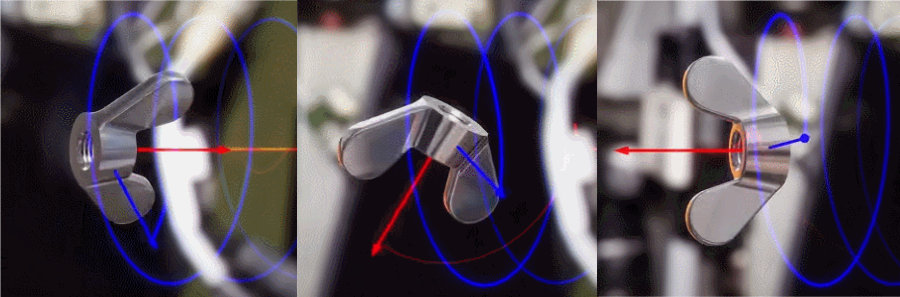
\includegraphics[width=0.9\textwidth]{dzhani.jpg}
\end{center}
   \caption{Một mô tả về hiệu ứng Dzhanibekov \cite{28}.}
\label{fig:10}
\end{figure*}

Nguyên lý đằng sau sự thay đổi nhanh chóng trục quay của Trái Đất nằm ở vật lý của các vật thể quay. Ví dụ kinh điển của hiện tượng này là hiệu ứng Dzhanibekov, được phát hiện bởi nhà du hành vũ trụ người Nga Vladimir Dzhanibekov \cite{37}, và được minh họa trong Hình \ref{fig:10}. Một vật thể không quay hoàn hảo quanh một trong ba trục quán tính chính sẽ không duy trì được một trục quay cố định. Nếu nó quay gần trục chính thứ hai, nó sẽ trải qua những sự thay đổi đột ngột trong chuyển động quay. Mặc dù đây không hoàn toàn là điều mà chúng ta tin là xảy ra trong các lần lật nhanh của Trái Đất, ý chính là khi không có tác động ngoại lực, chỉ có vật lý quay mới có thể giải thích sự thay đổi nhanh chóng trục quay của Trái Đất.

Cần lưu ý rằng Trái Đất gần như chắc chắn không trải qua một hiệu ứng Dzhanibekov đơn giản và đồng đều. Nếu điều này xảy ra, chúng ta sẽ có thể phát hiện sự thay đổi dần dần trục quay của Trái Đất theo thời gian. Thay vào đó, chúng tôi tin rằng Trái Đất trải qua những gián đoạn định kỳ, đột ngột trong cấu trúc vật lý của nó, dẫn đến sự tách rời giữa "vỏ ngoài quay" (vỏ/mantle) và "các phần quay bên trong" (lõi). Nếu không có tác động bên ngoài, định luật bảo toàn động lượng góc xác định rằng Trái Đất không thể tự nhiên thay đổi trục quay một cách đột ngột, nên sự tách biệt giữa vỏ ngoài và phần quay bên trong là một trong những điều hiếm hoi, ngoại trừ va chạm từ bên ngoài lên Trái Đất, có thể gây ra hiện tượng lật nhào nhanh chóng và đột ngột.

Quá trình cụ thể thúc đẩy sự rối loạn bên trong của Trái Đất được cho là sự thay đổi pha trong cấu trúc của sắt tạo nên lõi Trái Đất (Hình \ref{fig:11}). Lõi trong chủ yếu là sắt đóng gói lục giác (Fe) \cite{141}. Khi hcp-Fe này bị biến đổi thành trạng thái kim loại lỏng, nó giải phóng động năng và bị đẩy vào lõi ngoài. Sự chuyển pha này làm giảm độ thấm từ của lõi, làm suy yếu trường từ trường địa từ, đồng thời giải phóng nhiệt, hình thành các cấu trúc LLVP (vùng cắt lớn vận tốc thấp) (Hình \ref{fig:12}) \cite{38} trong lớp mantle, và làm nóng bề mặt Trái Đất thông qua các đại dương sâu. Cả hai xu hướng này đều đã được ghi nhận rõ ràng trong vài thế kỷ gần đây và sẽ được bàn luận thêm trong bài báo này.

\begin{figure*}[t]
\begin{center}
% \fbox{\rule{0pt}{2in} \rule{.9\linewidth}{0pt}}
\includegraphics[width=1\textwidth]{layers.jpg}
\end{center}
   \caption{Minh họa các quá trình bên trong Trái Đất dẫn tới hiện tượng lật ECDO \cite{129}.}
\label{fig:11}
\end{figure*}


\begin{figure}[t]
\begin{center}
% \fbox{\rule{0pt}{2in} \rule{0.9\linewidth}{0pt}}
   \includegraphics[width=1\linewidth]{llvp.jpg}
\end{center}
   \caption{Hình ảnh chi tiết về LLVP dưới Nam Phi \cite{28}.}
\label{fig:12}
\label{fig:onecol}
\end{figure}


Quá trình tương tự này bên trong Trái Đất, xảy ra theo chiều ngược lại, cũng được cho là nguyên nhân thúc đẩy Trái Đất trở về trạng thái quay hiện tại của nó tương đối sớm sau khi sự đảo cực diễn ra.

\section{Bằng chứng về một sự đảo cực Trái Đất sắp xảy ra}

Có lý do mạnh mẽ để tin rằng chúng ta đang ở bờ vực của một lần đảo cực nữa của Trái Đất. Một thảm họa lớn chưa xảy ra trong nhiều thiên niên kỷ, đây là tần suất mà các sự kiện này dường như xảy ra dựa trên các ghi chép lịch sử và dữ liệu. Dữ liệu mạnh mẽ nhất ủng hộ một lần đảo cực sắp tới đến từ dữ liệu địa từ gần đây, cho thấy từ trường Trái Đất đã suy yếu khoảng hai nghìn năm. Sự suy yếu này đã gia tăng nhanh chóng và đạt mức báo động trong vài thập kỷ gần đây.
Depicted in Figure \ref{fig:14} là trường từ trường trái đất vào năm 1590 và 2025 \cite{125,126}. Như thể hiện trong hình, trường này đã suy yếu đáng kể.

Một chỉ số khác cho sự suy yếu của trường từ trường là vị trí của cực bắc từ (Hình \ref{fig:13}). Trước đây, cực bắc từ chủ yếu nằm ở Bắc Cực của Canada. Tuy nhiên, trong vài thế kỷ qua, nó đã di chuyển chậm, và tăng tốc đáng kể trong vài thập kỷ gần đây. Hiện tại, nó đang di chuyển nhanh về phía Nga với tốc độ 55 km mỗi năm \cite{124}.

\begin{figure*}[t]
\begin{center}
% \fbox{\rule{0pt}{2in} \rule{.9\linewidth}{0pt}}
\includegraphics[width=0.9\textwidth]{saa.jpg}
\end{center}
   \caption{Hình minh họa sự suy yếu của trường từ trường trái đất từ năm 1590 đến 2025. Được tính toán bằng các mô hình gufm1 và IGRF-14 \cite{125,126}.}
\label{fig:14}
\end{figure*}

\begin{figure}[t]
\begin{center}
% \fbox{\rule{0pt}{2in} \rule{1\linewidth}{0pt}}
   \includegraphics[width=1\linewidth]{npw.jpg}
\end{center}
   \caption{Vị trí của cực bắc từ từ năm 1590 đến 2025, được thể hiện theo khoảng thời gian 5 năm \cite{142}.}
\label{fig:13}
\label{fig:onecol}
\end{figure}

\begin{figure}[t]
\begin{center}
% \fbox{\rule{0pt}{2in} \rule{1\linewidth}{0pt}}
   \includegraphics[width=1\linewidth]{ocean-highlight.jpg}
\end{center}
   \caption{Tốc độ ấm lên của đại dương sâu ($>$2000 m độ sâu) từ năm 1991 đến 2010, được khoanh tròn màu đỏ \cite{132}.}
\label{fig:15}
\label{fig:onecol}
\end{figure}

Trường từ của Trái Đất được cho là được tạo ra bởi một dynamo bên trong - những cột dòng dung nham chuyển động vòng tròn trong lõi ngoài của Trái Đất do sự quay của nó \cite{123}. Sự suy yếu của từ trường là triệu chứng của các rối loạn sâu bên trong Trái Đất. Theo lý thuyết ECDO, những rối loạn này giải phóng nhiệt và cuối cùng dẫn đến sự tách rời giữa lớp phủ và lõi, gây ra sự lật ngược của Trái Đất \cite{1}.

Có rất nhiều dữ liệu xác nhận sự tồn tại của các quá trình tỏa nhiệt bên trong Trái Đất. Trái Đất ấm lên được ghi nhận qua nhiệt độ bề mặt đại lục và đại dương tăng dần \cite{127,128}, nồng độ CO2 khí quyển tăng song hành cùng các luồng nhiệt từ Trái Đất \cite{129,130}, và sự suy giảm diện tích băng biển toàn cầu \cite{131}. Dữ liệu cho thấy mức CO2 và nhiệt độ tăng không phải là nguyên nhân của biến đổi khí hậu do con người mà là hệ quả sau cùng của một lõi Trái Đất tỏa nhiệt \cite{129}.

Đáng chú ý nhất, các nghiên cứu về tốc độ ấm lên ở đại dương sâu (độ sâu $>$2000 mét) cho thấy không chỉ các đại dương sâu đang ấm lên, mà tốc độ ấm mạnh nhất lại nằm ở lớp vực thẳm (4000 - 6000 m). Sự ấm lên ở đáy đại dương này có trung tâm bên dưới 4000 mét \cite{132,129}, điều này sẽ không thể xảy ra nếu các đại dương được làm nóng từ phía trên bởi khí quyển. Những dữ liệu này cho thấy bằng chứng mạnh mẽ rằng các biến đổi khí hậu và từ trường gần đây được dẫn dắt bởi các quá trình diễn ra sâu bên trong Trái Đất. Hình \ref{fig:15} thể hiện tốc độ ấm lên toàn cầu của đại dương sâu từ năm 1991 đến 2010 \cite{132}.

\section{Mô hình hóa Sự Lật Ngược Sắp Tới của Trái Đất}
\begin{figure}[b]
\begin{center}
% \fbox{\rule{0pt}{2in} \rule{1\linewidth}{0pt}}
   \includegraphics[width=1\linewidth]{saa-crop.jpeg}
\end{center}
   \caption{Một phép tính điểm bùng phát dựa trên Dị thường Nam Đại Tây Dương chỉ ra một ngày là 13 tháng 3, 2059 \cite{125,126}.}
\label{fig:16}
\label{fig:onecol}
\end{figure}

Dự đoán thời điểm khi Trái Đất lật tiếp theo là một nhiệm vụ phức tạp. Hiện nay, mô hình tốt nhất mà chúng ta có cho việc này nằm ở trường địa từ của Trái Đất - Dị thường Nam Đại Tây Dương (SAA). Khu vực này phía trên Nam Đại Tây Dương có cường độ trường địa từ yếu nhất và được xác định là vùng có cường độ trường dưới 32.000 nanoTesla \cite{135}, đây là giá trị trường yếu nhất vào năm 1590. Diện tích bề mặt của Dị thường Nam Đại Tây Dương đã tăng từ 1\% diện tích bề mặt Trái Đất vào năm 1590 lên 21\% vào năm 2025 \cite{136}.

Để ước tính khi nào Trái Đất có thể lật, tôi đã khớp dữ liệu về diện tích bề mặt SAA với một phương trình điểm bùng phát hàm mũ, mô hình hóa một hệ thống phức tạp khi đến gần chuyển tiếp tới hạn, lúc đó hệ thống sẽ trải qua sự thay đổi đột ngột và mạnh mẽ. Các phép tính của tôi đưa ra một ngày dự đoán điểm bùng phát là 13 tháng 3 năm 2059 (Hình \ref{fig:16}). Dự đoán này sẽ càng chính xác hơn khi ta tiến gần đến thời điểm chuyển tiếp \cite{136}.

Các chỉ số khác như độ dao động của trục quay, các bất thường thời tiết, và dữ liệu động đất và núi lửa cũng có thể giúp chúng ta có dự đoán tốt hơn về khi nào lần lật tiếp theo của Trái Đất có thể xảy ra.

\section{Dòng thời gian lịch sử ECDO}

Trong khi việc xác lập một mốc thời gian chính xác cho các sự kiện ECDO trong quá khứ là điều khó khăn, có vẻ như đã có ít nhất 2 sự kiện ECDO trong thời kỳ Holocene. Hãy lưu ý tới ghi chép của Herodotus từ các tu sĩ Ai Cập rằng, \textit{"từ vị vua đầu tiên cho tới vị tu sĩ Hephaistos cai trị cuối cùng này, đã có ba trăm bốn mươi mốt thế hệ người... Trong thời gian này họ nói rằng mặt trời đã di chuyển bốn lần khỏi vị trí mọc quen thuộc của nó, và nơi hiện nay nó lặn thì trước đây nó đã hai lần mọc lên, và nơi mà hiện nay nó mọc thì trước đây nó cũng đã hai lần lặn"} \cite{32}. Plato, người sống vào thế kỷ thứ năm TCN \cite{111}, từng phát biểu rằng sau trận lụt đã nhấn chìm Atlantis chỉ trong một ngày một đêm 9.000 năm trước, \textit{"từ đó tới nay đã có nhiều trận đại hồng thủy, và những người sót lại ở vùng núi không hiểu biết về chữ viết, trong suốt nhiều thế hệ chỉ tập trung vào việc mưu sinh"} \cite{112}, điều này cho thấy có thể đã xảy ra hơn hai lần lật kể từ cuối Younger Dryas khoảng năm 9700 TCN. Các bằng chứng vật lý được trình bày trong toàn bộ bài báo này và trong nghiên cứu của tôi \cite{2} cung cấp đầy đủ chứng cứ cho ghi chép của Plato.
Ứng viên gần đây nhất cho một lần lật ECDO là trong giai đoạn từ năm 2300 đến 1600 TCN, mà nhiều ghi chép về đại hồng thuỷ (Gun-Yu \cite{113,114,115}, Ogyges \cite{116,117}, Peru \cite{118,119}, Exodus \cite{120}), sự hủy diệt và bỏ hoang các nền văn minh (Mohenjo-Daro \cite{121}, Minoan Crete\cite{100,101}) và các hiện tượng vật lý bất thường (sự kiện bond \cite{122}, sự kiện 4.2 kilonăm \cite{90}) đã được xác định niên đại. Không có sự hội tụ bằng chứng đầy đủ nào gần đây hơn cho thấy một sự kiện thảm họa lớn.

\section{Kết luận}

Chiến dịch NANOOK là một nỗ lực trinh sát trong Chiến tranh Lạnh của Hoa Kỳ nhằm lập bản đồ Bắc Cực và bờ biển phía bắc Liên Xô sau Thế chiến II \cite{137}. Trong quá trình điều tra, họ phát hiện ra rằng cực từ nằm cách vị trí dự kiến dựa trên các phát hiện từ những chuyến thám hiểm trước đó từ 125 đến 200 dặm về phía bắc. Theo đó, \textit{"Giữa các nhà khoa học chính phủ, câu hỏi đặt ra là điều gì sẽ xảy ra khi cực từ và cực địa lý trùng nhau. Để trả lời, dưới sự kiểm soát dự án của Tiến sĩ Paul A. Siple, Rand Corporation đã được ký hợp đồng tiến hành các nghiên cứu trong phòng thí nghiệm sử dụng các mô hình trái đất được tạo thành từ các hình cầu đồng tâm – một hình cầu trong đại diện cho lõi sắt nóng chảy mang điện tích của trái đất, trục của nó xác định các cực “từ”; và một hình cầu ngoài đại diện cho lớp vỏ trái đất quay quanh một trục “địa lý”. Thông qua các thí nghiệm lặp đi lặp lại, xác định được rằng khi cực “từ” tiến gần cực “địa lý”, cực “từ” ở một điểm nào đó sẽ gia tốc tốc độ hội tụ như thể bị kéo về cực “địa lý” bởi lực hướng tâm và nhảy tới trùng nhau; nhưng thay vì trùng nhau, cực “từ” sẽ nhanh chóng “lật” quanh cực “địa lý”, sau đó xoay ra hướng xích đạo như thể do lực ly tâm, kết thúc tại vị trí hai trục tạo thành góc lệch xấp xỉ 89 độ. Sau khi hiện tượng “lật” cực này diễn ra, các trục cực dần dần hội tụ lại với nhau trong một khoảng thời gian dài"} \cite{138,139}.

Sau đó, \textit{"Tại một cuộc họp khoa học mà Thiếu tá White tham dự ở Lầu Năm Góc vào đầu năm 1948, các nhà khoa học đã thảo luận về việc có nên cảnh báo công chúng về hiện tượng lật cực sắp tới hay không. Không ai trong số các nhà khoa học đồng ý giữ kín thông tin đối với công chúng; tuy nhiên, họ cũng không thống nhất được cách công bố ra sao. Kiến thức về hiện tượng này, một số người cảm thấy, có thể tự nó phá hủy nền đạo đức xã hội. Nhưng nỗi lo sợ đó dường như không có cơ sở khi vào đầu những năm 1950, thông tin về hiện tượng lật cực đã được công bố trên cả báo giấy lẫn tạp chí, nhưng bất ngờ thay lại không nhận được phản ứng gì từ một công chúng dường như sững sờ, khép kín hoặc hoài nghi"} \cite{138,139}.

Tại sao chúng ta lại không chú ý tới điều này? Có nhiều lý do để tin rằng Trái Đất đã từng lật trước đây. Bài báo này, cùng với phần hai, cung cấp một bản tóm tắt súc tích về sự hội tụ lớn của bằng chứng từ nhiều lĩnh vực cho thấy điều này là đúng, chẳng hạn như các câu chuyện đại hồng thủy khắp thế giới, hóa thạch muối và sinh vật biển phủ khắp lục địa, các hầm trú ẩn cổ xưa dưới lòng đất, hài cốt động vật, và cảnh quan địa chất thảm khốc. Con người được cho là xuất hiện từ hàng trăm nghìn năm trước, nhưng lịch sử hiện đại chỉ kéo dài vài nghìn năm. Liệu có thể là cứ sau một khoảng thời gian, Trái Đất lại lật, các lục địa bị xóa sạch, và chúng ta buộc phải bắt đầu lại từ đầu – thời Đồ Đá – khiến những ghi chép về lịch sử cổ đại chỉ còn là một vài câu chuyện thảm họa? Nếu như vậy, thì ngăn ngừa điều này tái diễn có thể là một trong những nhiệm vụ quan trọng nhất của nhân loại.

Kết thúc, tôi xin để lại cho bạn ghi chép này trong Timaeus, được Plato viết lại, về một cuộc trò chuyện giữa Solon, một quốc vụ khanh người Athens, và các tư tế Ai Cập \cite{140}: \textit{"Và vào một dịp, khi [Solon] muốn lôi kéo họ vào cuộc đối thoại về lịch sử cổ xưa, ông cố kể với họ truyền thuyết lâu đời nhất của chúng tôi, về Phoroneus, người được xem là người đầu tiên, và Niobe; ông tiếp tục kể về truyền thuyết Deucalion và Pyrrha sau Đại Hồng Thủy, và cách họ sống sót, cùng phả hệ của hậu duệ họ; và bằng cách kể về số năm của các sự kiện được nhắc tới, ông cố gắng tính toán các giai đoạn thời gian. Lúc đó một trong các tư tế, một cụ già lão luyện, nói rằng: “Hỡi Solon, Solon, các người Hy Lạp luôn là những đứa trẻ: không có cái gì gọi là Hy Lạp già.” Nghe vậy, ông hỏi, “Ngài muốn nói gì với câu đó?” Và vị tư tế đáp, “Tâm hồn các ngươi đều trẻ trung. Vì lẽ đó các ngươi không có lấy một niềm tin nào là cổ xưa và được truyền lại từ các truyền thống cũ, và cũng không có bất kỳ khoa học nào mang dấu vết của tuổi tác. Đó là lý do: Đã từng và sẽ còn xảy ra nhiều cuộc hủy diệt nhân loại, trong đó lớn nhất là do lửa và nước, và những cuộc nhỏ hơn bởi vô số hình thức khác. Thật vậy, câu chuyện được kể ở nước các ngươi cũng như ở chúng ta, rằng từng một lần Phaethon, con trai của Helios, điều khiển cỗ xe của cha mình, và vì không thể cầm lái cho đúng lộ trình nên đã đốt cháy mọi thứ trên mặt đất và bản thân chết bởi sét – câu chuyện đó, như được kể, mang dáng dấp truyền thuyết, nhưng sự thật nằm ở chỗ sự dịch chuyển của các thiên thể chuyển động quanh trái đất, và sự hủy diệt của những gì trên trái đất bởi ngọn lửa dữ, việc này lặp lại theo chu kỳ dài. Vào những thời điểm như vậy, tất cả những ai sống trên núi cao và vùng khô ráo chịu thiệt hại nhiều hơn những người sống gần sông hoặc biển; còn trường hợp của chúng ta, sông Nile cứu chúng ta bằng cách dâng nước lên cao – cũng như đã cứu theo các cách khác. Và khi, ở những kỳ khác, các vị Thần thanh lọc mặt đất bằng lũ lụt, mọi mục đồng, người chăn thả trên núi được cứu, nhưng những người sống ở thành phố các ngươi thì bị dòng nước cuốn trôi xuống biển; còn ở đất nước chúng tôi, không phải khi đó hay bất cứ lúc nào nước lại đổ từ trên xuống đồng ruộng, ngược lại nước thường dâng lên từ dưới lòng đất. Do đó, vì những lý do này, những gì được giữ lại ở đây được coi là cổ xưa nhất; sự thật là ở bất kỳ nơi nào không có quá nóng hoặc quá lạnh thì luôn tồn tại một giống người nào đó, khi nhiều, khi ít. Nếu có sự kiện nào cao quý hoặc vĩ đại hoặc nổi bật, dù xảy ra ở nước các người hay nước ta hoặc nơi khác mà chúng ta có biết, tất cả các sự kiện đó đều được ghi chép và lưu giữ từ xa xưa trong các đền thờ của chúng tôi; còn người các ngươi và những người khác thì mỗi lần đều vừa mới bắt đầu với chữ viết và các kỹ nghệ như những quốc gia văn minh yêu cầu, và khi, theo chu kỳ, nước lũ trời lại tràn xuống các ngươi như dịch bệnh, nó không để lại ai ngoài những người thất học và chưa văn minh, khiến các ngươi trẻ lại như xưa, không biết gì về những gì diễn ra ngày xưa ở vùng đất này hoặc chính ở nước mình. Chắc chắn những phả hệ mà vừa nãy ngươi kể, Solon, về người dân nước ngươi, chẳng hơn gì truyện cổ của trẻ con; bởi trước tiên, ngươi chỉ nhớ một trận đại hồng thủy, dù thực tế đã có nhiều lần; kế đến, ngươi không biết rằng chủng tộc cao quý nhất và hoàn hảo nhất từng được sinh ra ở vùng đất mà ngươi đang sống, cả ngươi và toàn bộ thành phố hiện tại đều là hậu duệ từ hạt giống nhỏ còn sót lại đó; nhưng điều này đã bị ngươi bỏ lỡ vì qua nhiều thế hệ, những người sống sót đều chết mà không để lại gì bằng chữ viết. Thật vậy, đã từng một thời, Solon ạ, trước đợt hủy diệt lớn nhất bởi nước, Nhà nước Athens nay từng là mạnh mẽ nhất trong chiến tranh và tổ chức tốt nhất về mọi mặt. Người ta nói rằng họ đã sở hữu những tác phẩm nghệ thuật rực rỡ nhất và thể chế cao quý nhất dưới bầu trời mà chúng ta từng nghe kể”}.

Cũng những vị tư tế này, dĩ nhiên, còn kể cho Solon về nền văn minh cổ đại Atlantis: \textit{"Tất cả những gì chúng tôi có ở đây, nằm trong cửa sông mà chúng tôi nhắc đến, rõ ràng là một cảng có lối vào hẹp; nhưng phía xa kia là một đại dương thực sự, và vùng đất bao quanh nó xứng đáng nhất được gọi là lục địa thực sự, trọn vẹn và đúng nghĩa. Ở đảo Atlantis này từng tồn tại một liên minh các vị vua, quyền lực lớn lao và kỳ diệu, cai trị toàn bộ hòn đảo cùng với nhiều hòn đảo khác và một phần lục địa; hơn nữa, ở vùng đất trong Eo Biển, họ cai trị Libya đến tận Ai Cập, và châu Âu đến tận Tyrrhenia. Đoàn quân ấy, sau khi tập hợp, đã cố gắng trong một trận đánh duy nhất để bắt nước các ngươi và nước chúng ta cùng toàn bộ lãnh thổ phía trong Eo Biển làm nô lệ. Chính lúc đó, Solon ạ, người dân nước các ngươi đã tỏ ra xuất sắc về lòng dũng cảm và sức mạnh trước con mắt cả thế giới. Họ giữ vai trò lãnh đạo các bộ tộc Hy Lạp, khi thì đơn độc đứng vững dù bị cô lập, sau khi chạm trán những hiểm nguy chết người, đã đánh bại kẻ xâm lược và dựng bia chiến thắng; nhờ đó cứu thoát những ai chưa bị nô lệ hóa, và tất cả những ai sống trong ranh giới của Heracles đều được tự do một cách rộng lượng. Nhưng về sau đã xảy ra những trận động đất và lũ lụt khủng khiếp, một ngày và đêm tang thương đã đến, khi toàn bộ chiến binh của các ngươi bị đất nuốt chửng, và đảo Atlantis cũng vậy, bị biển nuốt chửng và biến mất"}.

\section{Lời cảm ơn}

Cảm ơn Ethical Skeptic, tác giả gốc của luận thuyết ECDO, vì đã hoàn thành luận án chuyên sâu, đột phá và chia sẻ nó với thế giới. Luận thuyết ba phần của ông \cite{1} vẫn là công trình nền tảng cho lý thuyết Dao động Dzhanibekov Tách rời Lõi-Manti Trái Đất (ECDO), và chứa nhiều thông tin hơn rất nhiều so với những gì tôi trình bày sơ lược ở đây.

Cảm ơn Ankit, người đã xử lý dữ liệu tổng hợp các thảm họa trong Bảng 1.
Và dĩ nhiên, xin cảm ơn những người khổng lồ mà chúng ta đang đứng trên vai họ; những người đã thực hiện tất cả các nghiên cứu và điều tra giúp cho công trình này trở nên khả thi và đã nỗ lực mang lại ánh sáng cho nhân loại.

\clearpage
\twocolumn

\section{Hình ảnh bổ sung}


\begin{figure}[H]
\begin{center}
% \fbox{\rule{0pt}{2in} \rule{1\linewidth}{0pt}}
   \includegraphics[width=1\linewidth]{wave.jpg}
\end{center}
   \caption{Cận cảnh sự xói mòn dạng sóng parabol, khoét sâu dưới chân trên kim tự tháp Khafre \cite{27}.}
\label{fig:19}
\label{fig:onecol}
\end{figure}

\begin{figure}[H]
\begin{center}
% \fbox{\rule{0pt}{2in} \rule{1\linewidth}{0pt}}
   \includegraphics[width=1\linewidth]{star-stone.jpg}
\end{center}
   \caption{Bản đồ các vì sao được khắc lên đá trong một trong các đường hầm của kim tự tháp Khufu \cite{28}.}
\label{fig:20}
\label{fig:onecol}
\end{figure}

\begin{figure*}[t]
\begin{center}
% \fbox{\rule{0pt}{2in} \rule{.9\linewidth}{0pt}}
\includegraphics[width=1\textwidth]{deepsea.jpg}
\end{center}
   \caption{Hình ảnh trực quan về dị thường nhiệt đại dương ở tầng sâu và vực thẳm so với đường cong nhiệt đại dương thông thường của khí quyển. Dị thường nhiệt tổng thể được lấy từ NOAA \cite{147}, phân bố nhiệt sâu và vực thẳm từ nghiên cứu của Desbruyeres \cite{132}, và quá trình xử lý dữ liệu cũng như trực quan hóa được thực hiện bởi Ethical Skeptic \cite{129}.}
\label{fig:21}
\end{figure*}

\begin{figure*}[t]
\begin{center}
% \fbox{\rule{0pt}{2in} \rule{.9\linewidth}{0pt}}
\includegraphics[width=1\textwidth]{sealevel.jpeg}
\end{center}
   \caption{Mực nước biển cho thấy phương sai tăng 20\% trong vòng 75 năm tại 63 trạm quan trắc, cho thấy tốc độ dòng chảy đã tăng lên. Sự gia tăng phương sai mực nước biển xảy ra đồng thời với các đợt xung nhiệt đại dương, cho thấy cả hai có thể đều do hiện tượng làm nóng từ sâu dưới đáy đại dương của Trái Đất \cite{2,129}.}
\label{fig:22}
\end{figure*}

\begin{figure*}[t]
\begin{center}
% \fbox{\rule{0pt}{2in} \rule{.9\linewidth}{0pt}}
\includegraphics[width=1\textwidth]{co2.jpg}
\end{center}
   \caption{Nồng độ CO2 trong khí quyển (ppm) đã tăng đều đặn trong 45 năm qua, có thể do nhiệt độ đại dương tăng lên. Nguồn: NOAA \cite{148,129}.}
\label{fig:23}
\end{figure*}

\begin{figure*}[t]
\begin{center}
% \fbox{\rule{0pt}{2in} \rule{.9\linewidth}{0pt}}
\includegraphics[width=1\textwidth]{ice.jpg}

\end{center}
   \caption{Diện tích băng biển toàn cầu đã giảm trong 45 năm qua, do Trái Đất ấm lên. Nguồn: ADS \cite{149}.}
\label{fig:24}
\end{figure*}

\clearpage
\twocolumn

{\small
\bibliographystyle{ieee}
\bibliography{egbib}
}

\end{document}